\section{Cell Error}
Once the Voronoi tessellation has been determined, it is re-centred based on the weighted average of the points in the cell. Sources are added to cells by determining the cell centre which is closest to it using the standard distance equation:
\begin{equation}
d = \sqrt{(x_i - x_j)^2 + (y_i - y_j)^2},
\end{equation}
where $(x_i,y_i)$ is the location of a source in the plane and $(x_j,y_j)$ is the location of a centre. The closest centre is such that $d$ is minimum. For each source, $s_i$ we therefore seek its minimum distance, $d_i$, such that for a set of $n$ centres:
\begin{equation}
d_i = \min^n_j \sqrt{(x_i - x_j)^2 + (y_i - y_j)^2}.
\end{equation}
This is done to add the influence of weaker sources in the overall correction and is especially necessary when the cell is generated by a source slightly above the intensity threshold and contains a source slightly below the threshold. We seek a new weighted centre such that the error for a cell is minimum. The error for a cell containing $N$ sources is defined as
\begin{equation} \label{eq:cellerr}
	\epsilon_j = \sum^N_{i=1} z_i||\vec{x_i} - \vec{x_j}||^2,
\end{equation}
where $\vec{x_i} = (x_i,y_i)$ is the location, $z_i$ is the intensity of some source in the cell, and $\vec{x_j}$ is the location of the new centre. 
\\
\\
This error function has a local minimum at the point where its derivative with regard to $\vec{x_j}$ is zero, or
\begin{align*}
	\frac{d\epsilon}{d\vec{x_j}} &= \sum^N_{i=1} \frac{d}{d\vec{x_j}}z_i(||\vec{x_i}||^2 -2\vec{x_i}\cdot\vec{x_j} + ||\vec{x_j}||^2) \\
	&= \sum^N_{i=1} z_i(2\vec{x_i} - 2\vec{x_j}) = 0 \\
\end{align*}
or
\begin{equation*}
	2\sum^N_{i=1} z_i\vec{x_i} = 2\sum^N_{i=1}z_i\vec{x_j}.
\end{equation*}
Since $\vec{x_j}$ is not dependent on the sum, it can be removed and the equation reordered to give
\begin{equation}
	\vec{x_j} = \frac{\sum^N_{i=1} z_i\vec{x_i}}{\sum^N_{i=1}z_i}.
\end{equation}
From this, the new centre is determined. The intensity of the centre is determined as the sum of the intensities in the cell, or:
\begin{equation}
	z_j = \sum^N_{i=1} z_i.
\end{equation}
Once the cell's new centre has been obtained, its error is calculated using Equation (\ref{eq:cellerr}). An example of centre correction can be seen in the transition from Figure \ref{fig:recen1} to Figure \ref{fig:recen2}.
\begin{figure}[H]
  \centering
  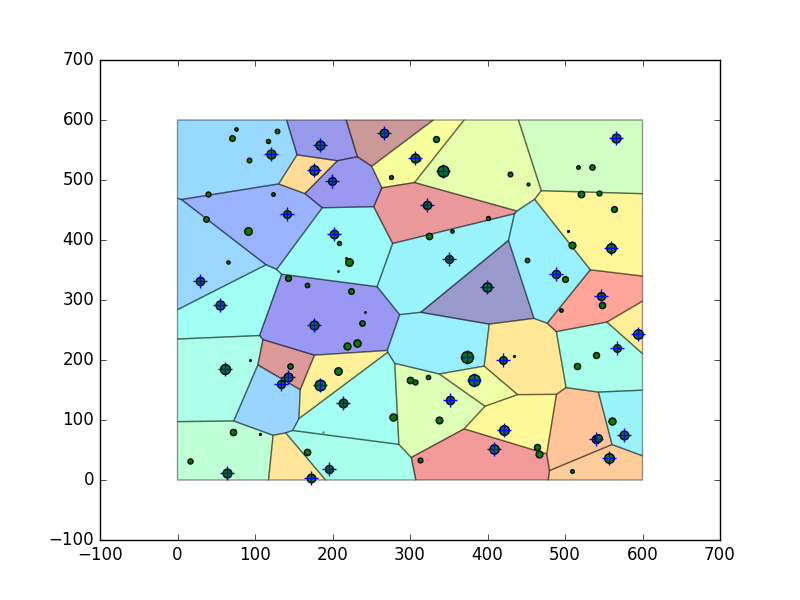
\includegraphics[width=0.8\textwidth]{Images/recentre1.png}
  \caption{Tessellation with high intensity sources as centres.}
  \label{fig:recen1}
\end{figure}
\begin{figure}[H]
  \centering
  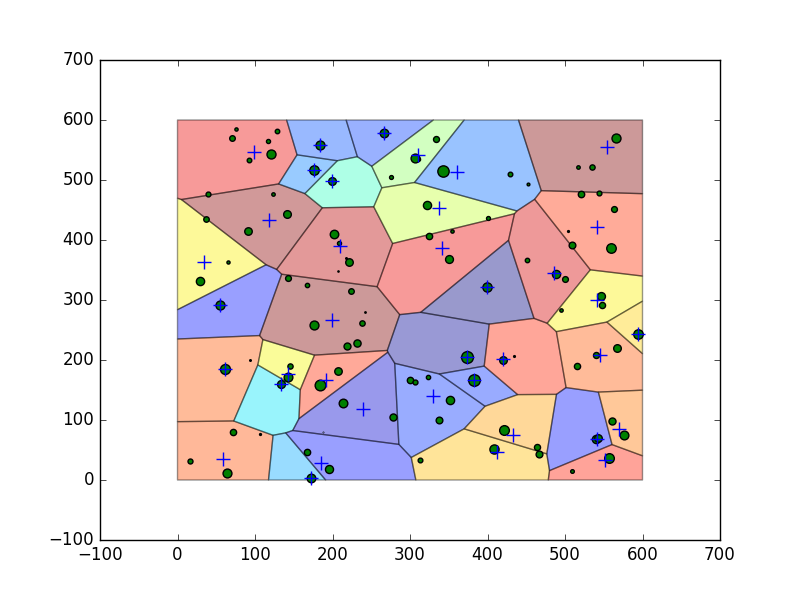
\includegraphics[width=0.8\textwidth]{Images/recentre2.png}
  \caption{Tessellation with the weighted average of the sources in the cells as their centres.}
  \label{fig:recen2}
\end{figure}